%%%%%%%%%%%%%%%%%%%%%%%%%%%%%%%%%%%%%%%%%
% Beamer Presentation
% LaTeX Template
% Version 1.0 (10/11/12)
%
% This template has been downloaded from:
% http://www.LaTeXTemplates.com
%
% License:
% CC BY-NC-SA 3.0 (http://creativecommons.org/licenses/by-nc-sa/3.0/)
%
%%%%%%%%%%%%%%%%%%%%%%%%%%%%%%%%%%%%%%%%%

%----------------------------------------------------------------------------------------
%	PACKAGES AND THEMES
%----------------------------------------------------------------------------------------

\documentclass[handout]{beamer}

\mode<presentation> {

% The Beamer class comes with a number of default slide themes
% which change the colors and layouts of slides. Below this is a list
% of all the themes, uncomment each in turn to see what they look like.

%\usetheme{default}
%\usetheme{AnnArbor}
%\usetheme{Antibes}
%\usetheme{Bergen}
%\usetheme{Berkeley}
%\usetheme{Berlin}
%\usetheme{Boadilla}
%\usetheme{CambridgeUS}
%\usetheme{Copenhagen}
%\usetheme{Darmstadt}
%\usetheme{Dresden}
%\usetheme{Frankfurt}
%\usetheme{Goettingen}
%\usetheme{Hannover}
%\usetheme{Ilmenau}
%\usetheme{JuanLesPins}
%\usetheme{Luebeck}
\usetheme{Madrid}
%\usetheme{Malmoe}
%\usetheme{Marburg}
%\usetheme{Montpellier}
%\usetheme{PaloAlto}
%\usetheme{Pittsburgh}
%\usetheme{Rochester}
%\usetheme{Singapore}
%\usetheme{Szeged}
%\usetheme{Warsaw}

% As well as themes, the Beamer class has a number of color themes
% for any slide theme. Uncomment each of these in turn to see how it
% changes the colors of your current slide theme.

%\usecolortheme{albatross}
%\usecolortheme{beaver}
%\usecolortheme{beetle}
%\usecolortheme{crane}
%\usecolortheme{dolphin}
%\usecolortheme{dove}
%\usecolortheme{fly}
%\usecolortheme{lily}
%\usecolortheme{orchid}
%\usecolortheme{rose}
%\usecolortheme{seagull}
%\usecolortheme{seahorse}
%\usecolortheme{whale}
%\usecolortheme{wolverine}

%\setbeamertemplate{footline} % To remove the footer line in all slides uncomment this line
%\setbeamertemplate{footline}[page number] % To replace the footer line in all slides with a simple slide count uncomment this line

%\setbeamertemplate{navigation symbols}{} % To remove the navigation symbols from the bottom of all slides uncomment this line
}

\usepackage{graphicx} % Allows including images
\usepackage{booktabs} % Allows the use of \toprule, \midrule and \bottomrule in tables
\usepackage{cool}
\usepackage{tikz}
\usepackage{amsmath}
\DeclareMathOperator*{\argmax}{argmax}
\DeclareMathOperator*{\argmin}{argmin}
\usetikzlibrary{positioning}

%----------------------------------------------------------------------------------------
%	TITLE PAGE
%----------------------------------------------------------------------------------------

\title[Utility Theory]{Understanding Risk-Aversion through Utility Theory} % The short title appears at the bottom of every slide, the full title is only on the title page

\author{Ashwin Rao} % Your name
\institute[Stanford] % Your institution as it will appear on the bottom of every slide, may be shorthand to save space
{
ICME, Stanford University
 % Your institution for the title page
}

\date{\today} % Date, can be changed to a custom date

\begin{document}
\begin{frame}
\titlepage % Print the title page as the first slide
\end{frame}

\begin{frame}
\frametitle{Intuition on Risk-Aversion and Risk-Premium}
\pause
\begin{itemize}[<+->]
\item Let's play a game where your payoff is based on outcome of a fair coin
\item You get \$100 for HEAD and \$0 for TAIL
\item How much would you pay to play this game?
\item You immediately say: ``Of course, \$50''
\item Then you think a bit, and say: ``A little less than \$50''
\item Less because you want to ``be compensated for taking the risk''
\item The word {\em Risk} refers to the degree of variation of the outcome
\item We call this risk-compensation as {\bf Risk-Premium}
\item Our {\em personality-based} degree of risk fear is known as {\bf Risk-Aversion}
\item So, we end up paying \$50 minus Risk-Premium to play the game
\item {\bf Risk-Premium grows with Outcome-Variance \& Risk-Aversion}
\end{itemize}
\end{frame}

\begin{frame}
\frametitle{Specifying Risk-Aversion through a Utility function}
\pause
\begin{itemize}[<+->]
\item We seek a ``valuation formula'' for the amount we'd pay that:
\begin{itemize}
\item Increases one-to-one with the Mean of the outcome
\item Decreases as the Variance of the outcome (i.e.. Risk) increases
\item Decreases as our Personal Risk-Aversion increases
\end{itemize}
\item The last two properties above define the Risk-Premium
\item But fundamentally why are we Risk-Averse?
\item Why don't we just pay the mean of the random outcome?
\item {\bf Reason: Our satisfaction to better outcomes grows non-linearly}
\item We express this satisfaction non-linearity as a mathematical function
\item Based on a core economic concept called {\bf Utility of Consumption}
\item We will illustrate this concept with a real-life example
\end{itemize}
\end{frame}

\begin{frame}
\frametitle{Law of Diminishing Marginal Utility}
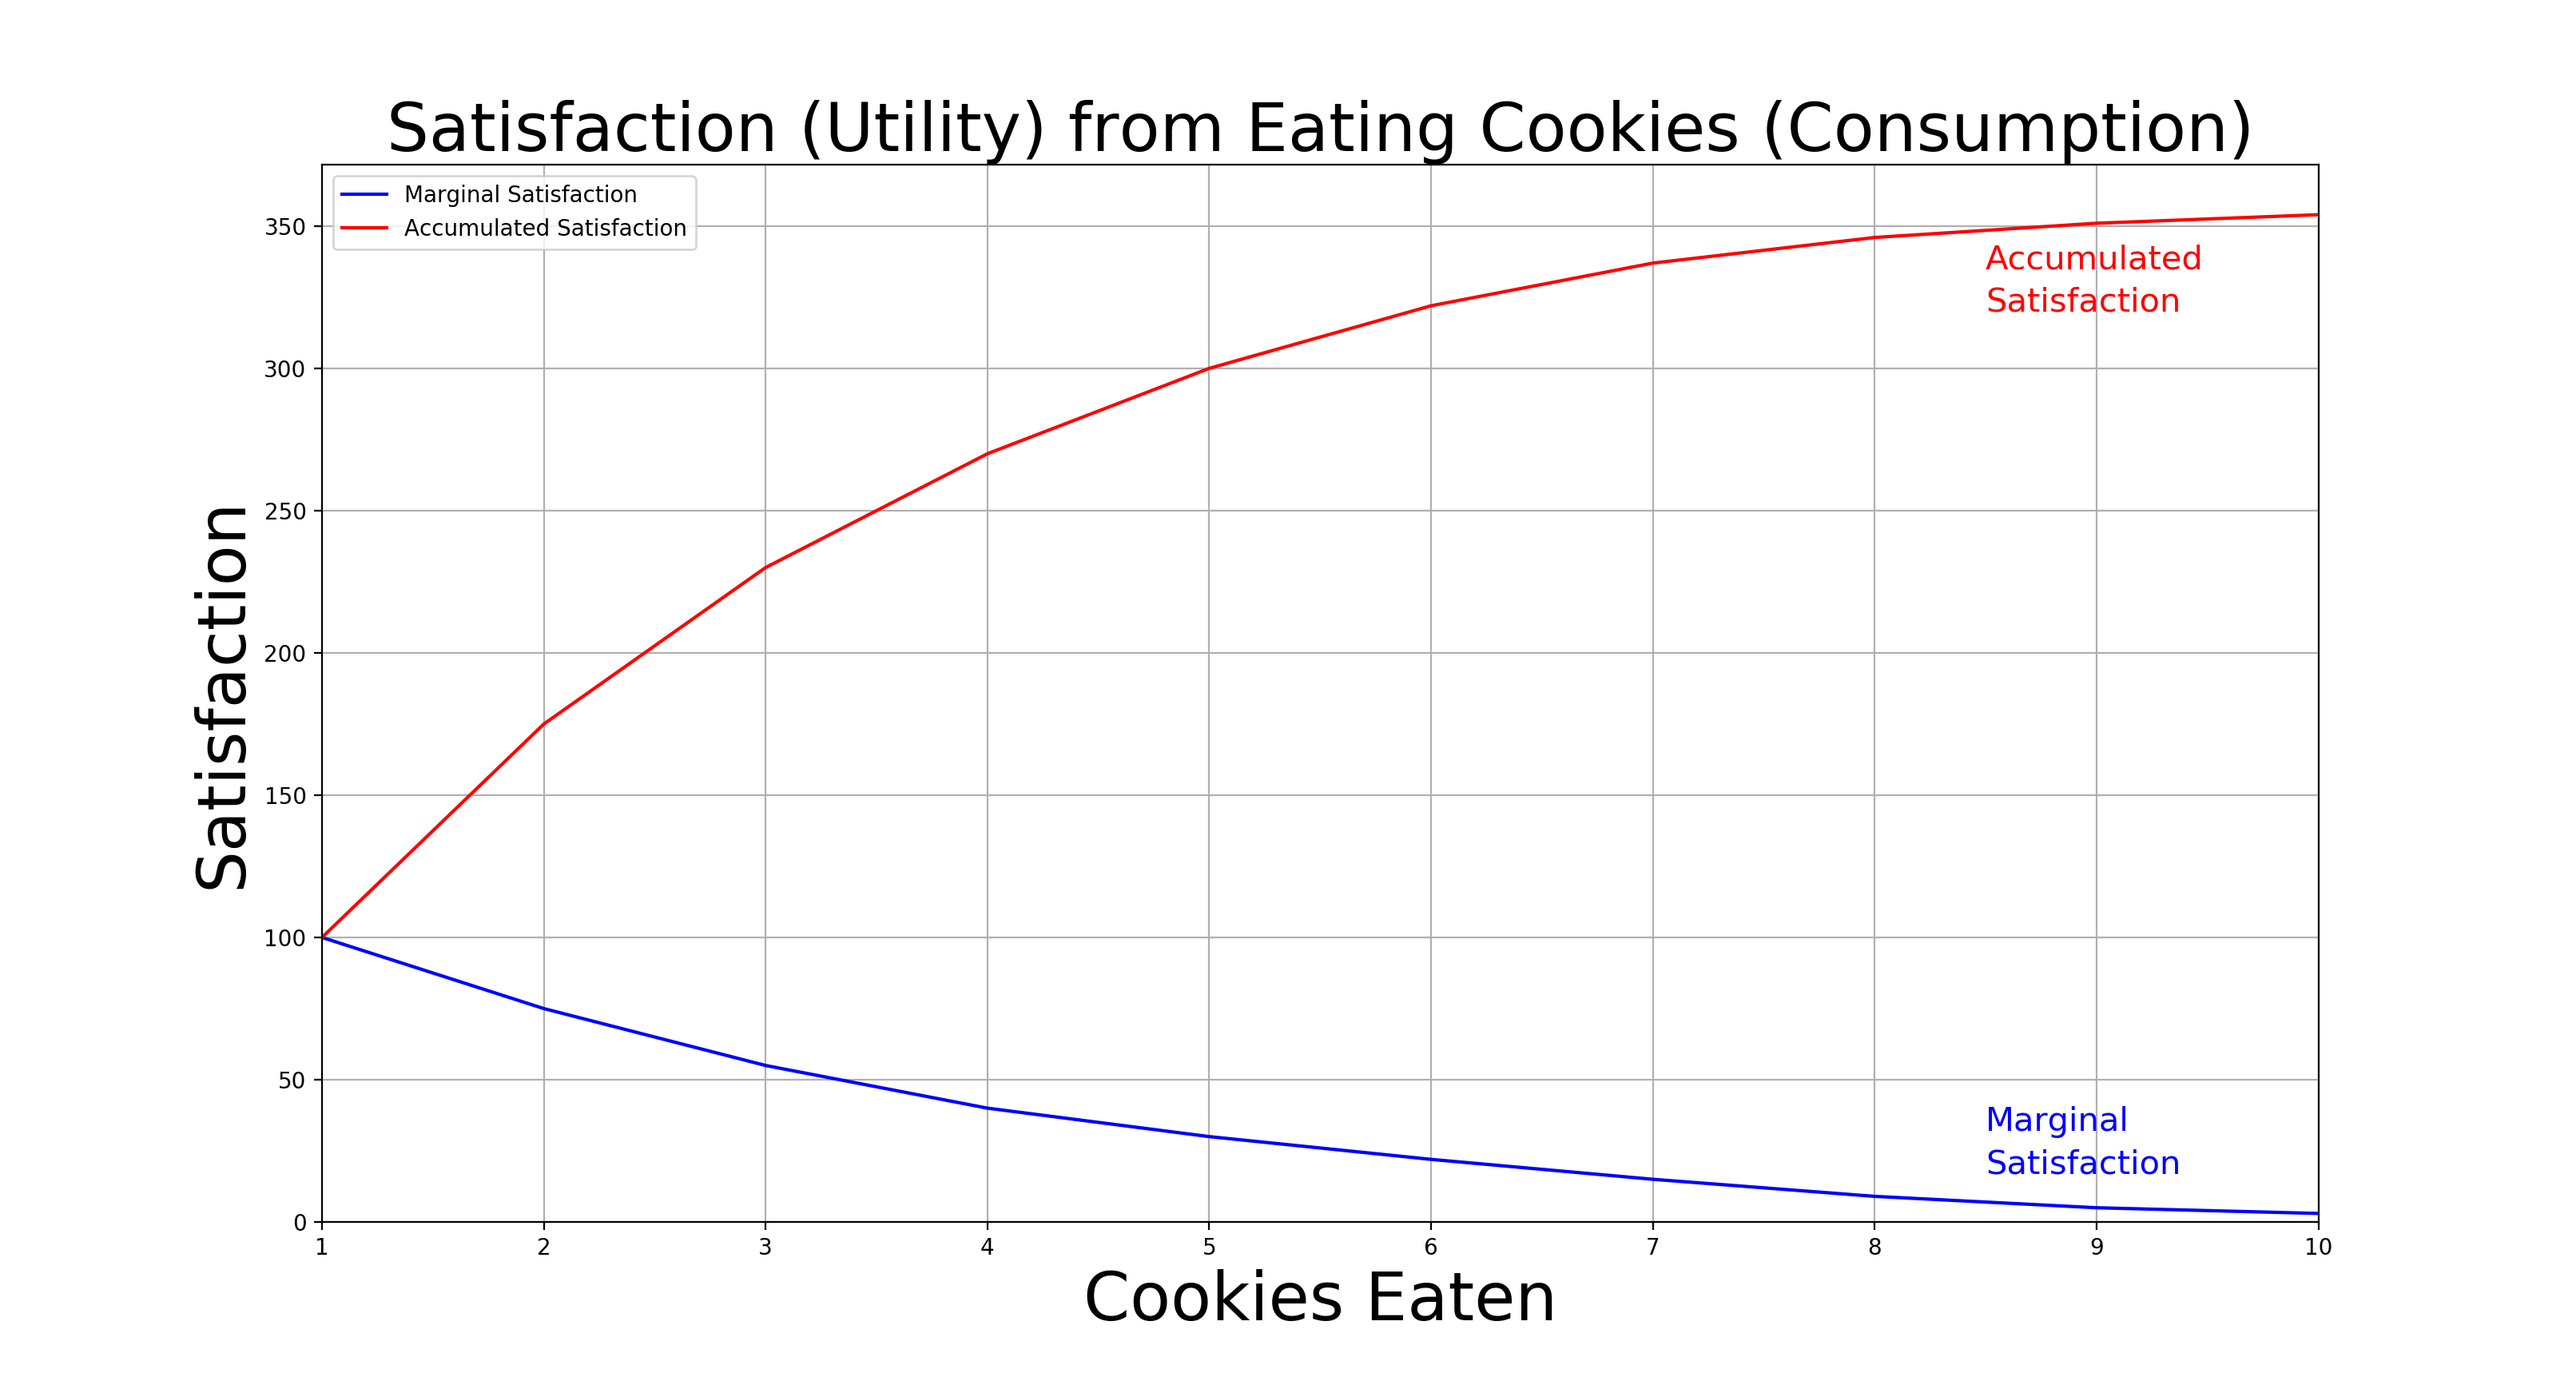
\includegraphics[scale=0.32]{utility.png}
\end{frame}

\begin{frame}
\frametitle{Utility of Consumption and Certainty-Equivalent Value}
\pause
\begin{itemize}[<+->]
\item Marginal Satisfaction of eating cookies is a diminishing function
\item Hence, Accumulated Satisfaction is a concave function
\item Accumulated Satisfaction represents Utility of Consumption $U(x)$
\item Where $x$ represents the uncertain outcome being consumed
\item Degree of concavity represents extent of our Risk-Aversion
\item Concave $U(\cdot)$ function $\Rightarrow \mathbb{E}[U(x)] <  U(\mathbb{E}[x])$
\item We define {\bf Certainty-Equivalent Value} $x_{CE} = U^{-1}(\mathbb{E}[U(x)])$
\item Denotes certain amount we'd pay to consume an uncertain outcome
\item {\bf Absolute Risk-Premium} $\pi_A = \mathbb{E}[x] - x_{CE}$
\item {\bf Relative Risk-Premium} $\pi_R = \frac {\pi_A} {\mathbb{E}[x]} = \frac{\mathbb{E}[x] - x_{CE}} {\mathbb{E}[x]} = 1 - \frac {x_{CE}} {\mathbb{E}[x]}$
\end{itemize}
\end{frame}

\begin{frame}
\frametitle{Certainty-Equivalent Value}
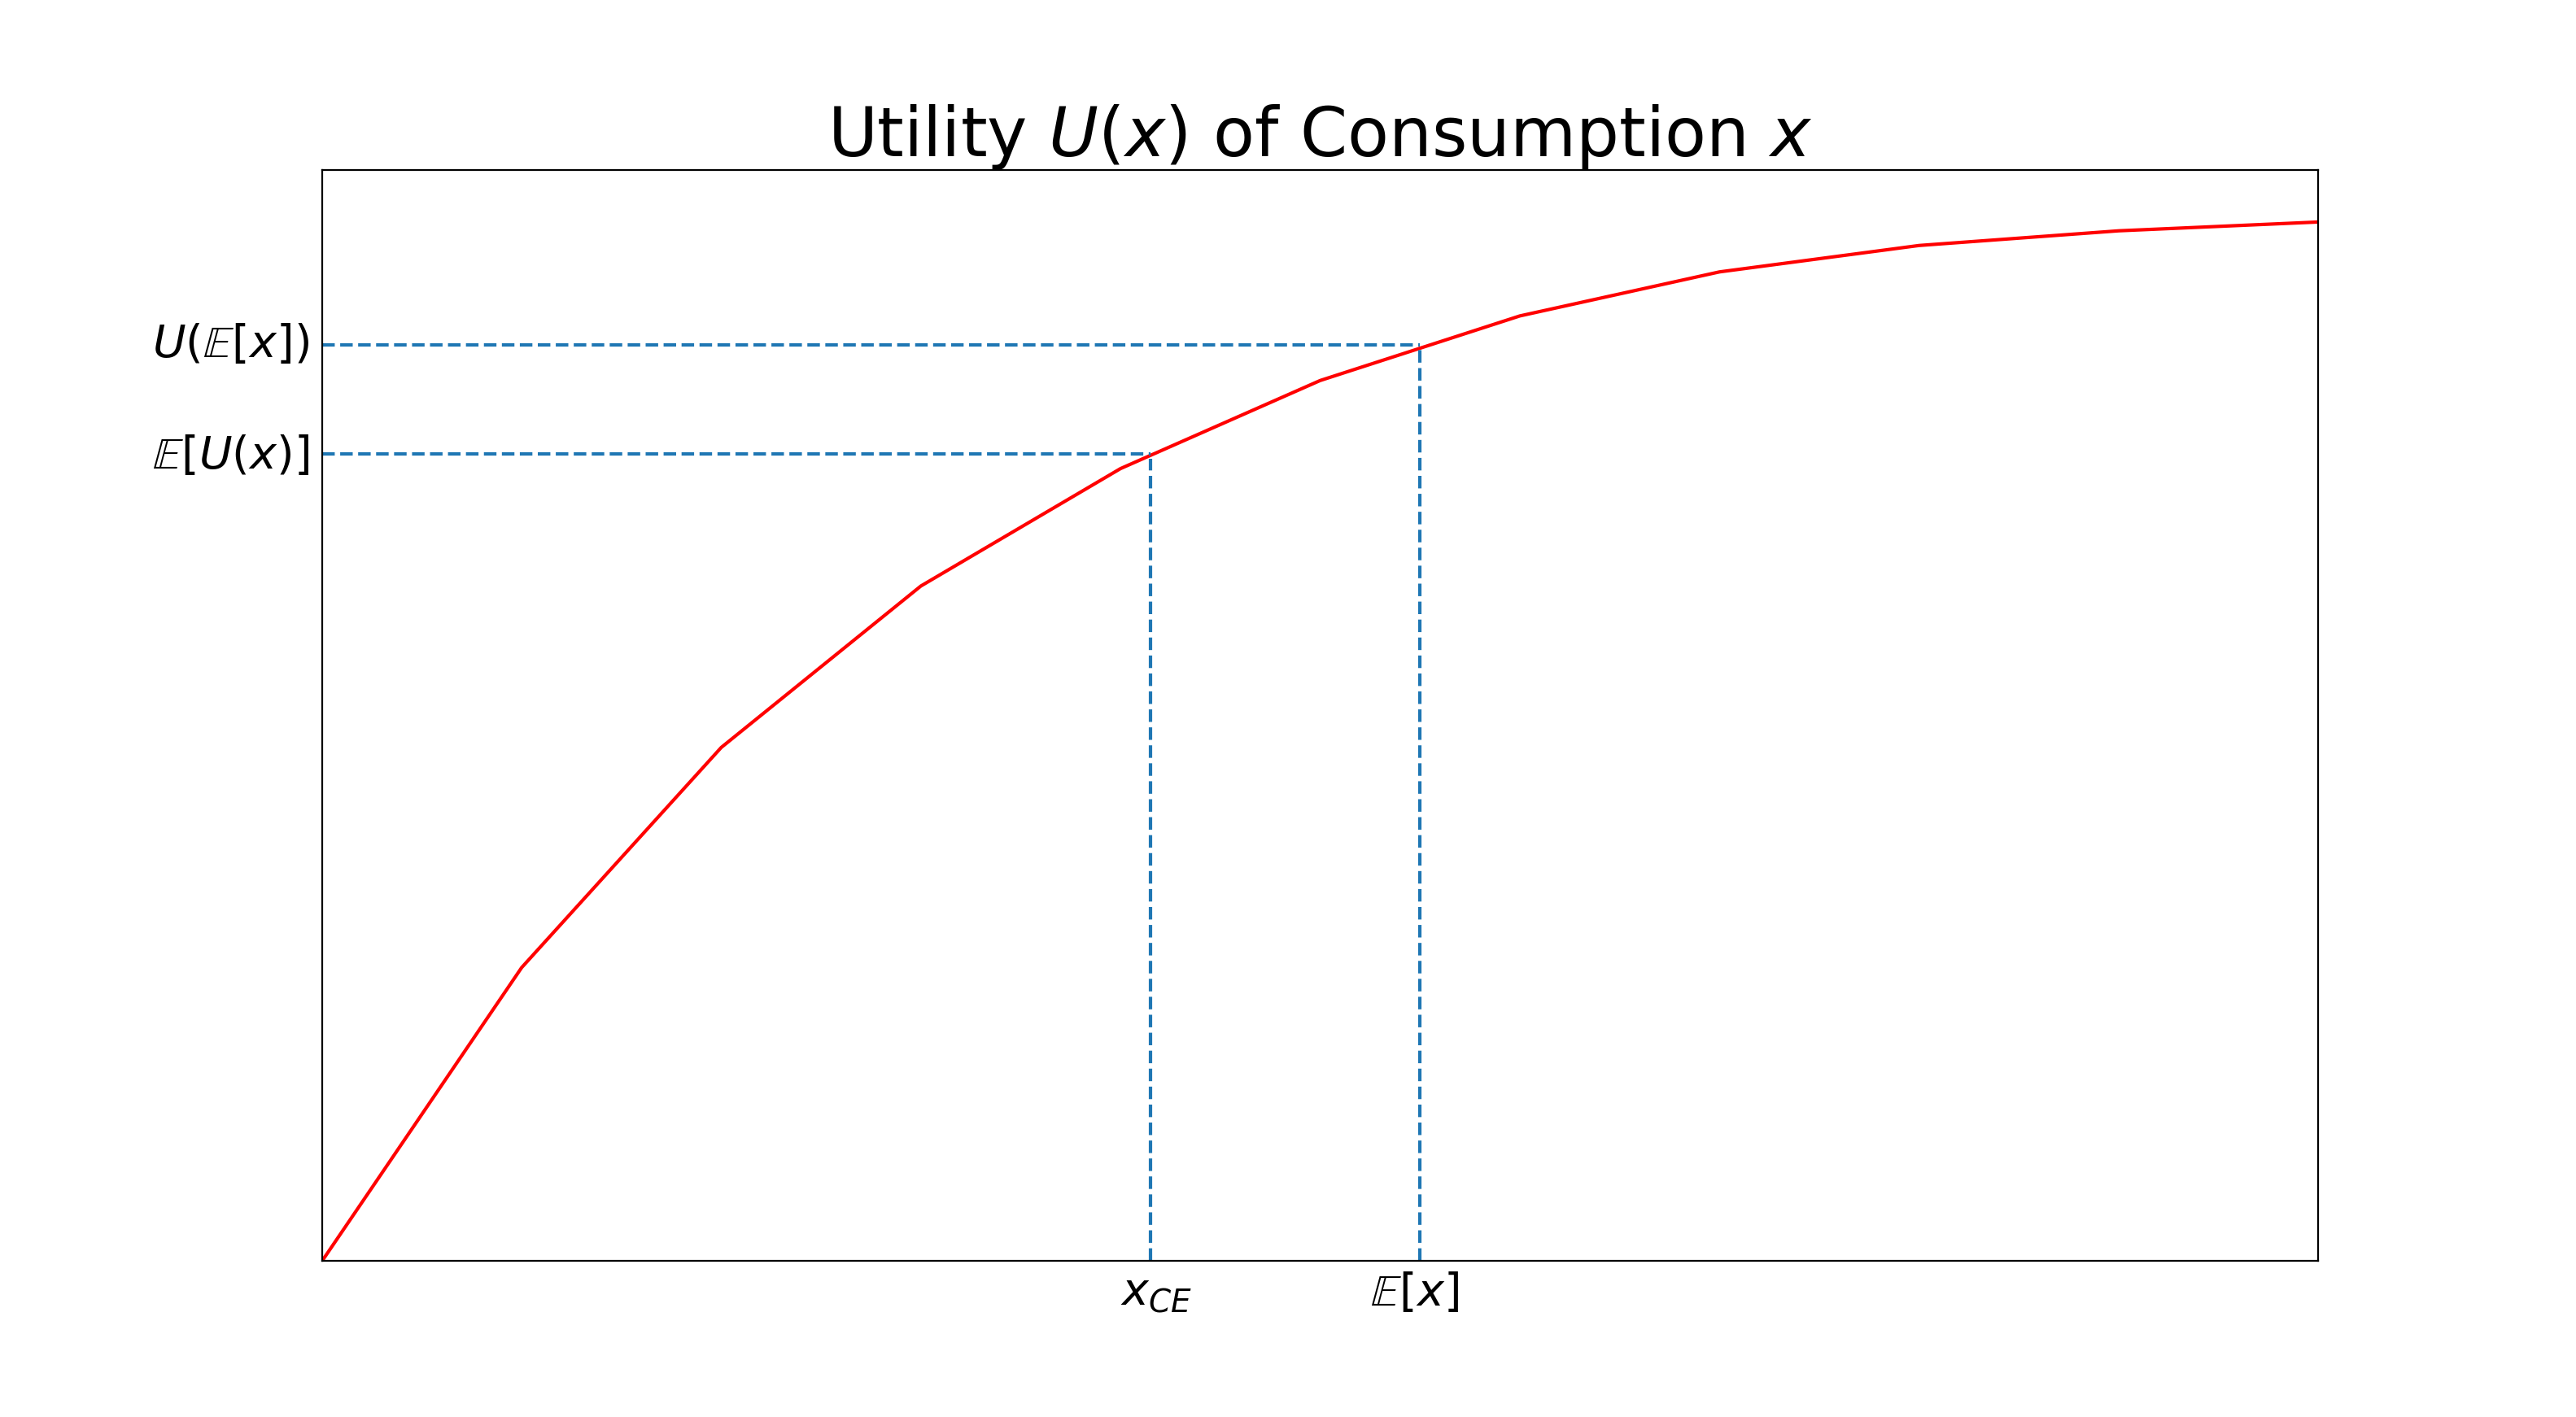
\includegraphics[scale=0.32]{ce.png}
\end{frame}

\begin{frame}
\frametitle{Calculating the Risk-Premium}
\pause
\begin{itemize}[<+->]
\item We develop mathematical formalism to calculate Risk-Premia $\pi_A, \pi_R$
\item To lighten notation, we refer to $\mathbb{E}[x]$ as $\bar{x}$ and Variance of $x$ as $\sigma_x^2$
\item Taylor-expand $U(x)$ around $\bar{x}$, ignoring terms beyond quadratic
$$U(x) \approx U(\bar{x}) + U'(\bar{x}) \cdot (x - \bar{x}) + \frac 1 2 U''(\bar{x}) \cdot (x - \bar{x})^2$$
\item Taylor-expand $U(x_{CE})$ around $\bar{x}$, ignoring terms beyond linear
$$U(x_{CE}) \approx U(\bar{x}) + U'(\bar{x}) \cdot (x_{CE} - \bar{x})$$
\item Taking the expectation of the $U(x)$ expansion, we get:
$$\mathbb{E}[U(x)] \approx U(\bar{x}) + \frac 1 2 \cdot U''(\bar{x}) \cdot \sigma_x^2$$
\item Since $\mathbb{E}[U(x)] = U(x_{CE})$, the above two expressions are $\approx$. Hence,
$$U'(\bar{x}) \cdot (x_{CE} - \bar{x}) \approx \frac 1 2 \cdot U''(\bar{x}) \cdot \sigma_x^2$$
\end{itemize}
\end{frame}

\begin{frame}
\frametitle{Absolute \& Relative Risk-Aversion}
\pause
\begin{itemize}[<+->]
\item From the last equation on the previous slide, Absolute Risk-Premium
$$\pi_A = \bar{x} - x_{CE} \approx - \frac 1 2 \cdot \frac {U''(\bar{x})} {U'(\bar{x})} \cdot \sigma_x^2$$
\item We refer to function A(x) = $-\frac {U''(x)} {U'(x)}$ as the {\bf Absolute Risk-Aversion}
$$\pi_A \approx \frac 1 2 \cdot A(\bar{x}) \cdot \sigma_x^2$$
\item In multiplicative uncertainty settings, we focus on variance $\sigma_{\frac x {\bar{x}}}^2$ of $\frac x {\bar{x}}$ 
\item In multiplicative settings, we also focus on Relative Risk-Premium $\pi_R$
$$\pi_R = \frac {\pi_A} {\bar{x}} \approx - \frac 1 2 \cdot \frac {U''(\bar{x}) \cdot \bar{x}} {U'(\bar{x})} \cdot \frac {\sigma_x^2} {\bar{x}^2} = - \frac 1 2 \cdot \frac {U''(\bar{x}) \cdot \bar{x}} {U'(\bar{x})} \cdot \sigma_{\frac x {\bar{x}}}^2$$
\item We refer to function R(x) = $-\frac {U''(x) \cdot x} {U'(x)}$ as the {\bf Relative Risk-Aversion}
$$\pi_R \approx \frac 1 2 \cdot R(\bar{x}) \cdot \sigma_{\frac x {\bar{x}}}^2$$
\end{itemize}
\end{frame}

\begin{frame}
\frametitle{Taking stock of what we're learning here}
\pause
\begin{itemize}[<+->]
\item We've shown that Risk-Premium can be expressed as the product of:
\begin{itemize}
\item Extent of Risk-Aversion: either $A(\bar{x})$ or $R(\bar{x})$
\item Extent of uncertainty of outcome: either $\sigma_x^2$ or $\sigma_{\frac {x} {\bar{x}}}^2$
\end{itemize}
\item We've expressed the extent of Risk-Aversion as the ratio of:
\begin{itemize}
\item Concavity of the Utility function (at $\bar{x}$): $-U''(\bar{x})$
\item Slope of the Utility function (at $\bar{x}$): $U'(\bar{x})$
\end{itemize}
\item For optimization problems, we ought to maximize $\mathbb{E}[U(x)]$ (not $\mathbb{E}[x])$
\item Linear Utility function $U(x) = a + b \cdot x$ implies {\em Risk-Neutrality}
\item Now we look at typically-used Utility functions $U(\cdot)$ with:
\begin{itemize}
\item Constant Absolute Risk-Aversion (CARA)
\item Constant Relative Risk-Aversion (CRRA)
\end{itemize}
\end{itemize}
\end{frame}

\begin{frame}
\frametitle{Constant Absolute Risk-Aversion (CARA)}
\pause
\begin{itemize}[<+->]
\item Consider the Utility function $U(x) = - e^{-ax}$
\item Absolute Risk-Aversion $A(x) = \frac {-U''(x)} {U'(x)} = a$
\item $a$ is called Coefficient of Constant Absolute Risk-Aversion (CARA)
\item If the random outcome $x \sim \mathcal{N}(\mu, \sigma^2)$,
$$\mathbb{E}[U(x)] = -e^{-a \mu + \frac {a^2 \sigma^2} 2}$$
$$x_{CE} = \mu - \frac {a \sigma^2} 2$$
$$\mbox{Absolute Risk Premium } \pi_A = \mu - x_{CE} =  \frac {a \sigma^2} 2$$
\item For optimization problems where $\sigma^2$ is a function of $\mu$, we seek the distribution that (approximately) maximizes $\mu - \frac {a \sigma^2} 2$
\end{itemize}
\end{frame}

\begin{frame}
\frametitle{Constant Relative Risk-Aversion (CRRA)}
\pause
\begin{itemize}[<+->]
\item Consider the Utility function $U(x) = \frac {x^{1 - \gamma}} {1 - \gamma}$ for $\gamma \neq 1$
\item Relative Risk-Aversion $R(x) = \frac {-U''(x) \cdot x} {U'(x)} = \gamma$
\item $\gamma$ is called Coefficient of Constant Relative Risk-Aversion (CRRA)
\item For $\gamma = 1$, $U(x) = \log(x)$ (note: $R(x) = \frac {-U''(x) \cdot x} {U'(x)} = 1$)
\item If the random outcome $x$ is lognormal, with $\log(x) \sim \mathcal{N}(\mu, \sigma^2)$,
$$
\mathbb{E}[U(x)] = 
\begin{cases}
\frac {e^{\mu (1 - \gamma) + \frac {\sigma^2} 2 (1-\gamma)^2}} {1 - \gamma} & \text{for } \gamma \neq 1\\
\mu & \text {for } \gamma = 1\\
\end{cases}
$$
$$x_{CE} = e^{\mu + \frac {\sigma^2} 2 (1- \gamma)}$$
$$\mbox{Relative Risk Premium } \pi_R = 1 - \frac {x_{CE}} {\bar{x}} =  1 - e^{-\frac {\sigma^2 \gamma} 2}$$
\end{itemize}
\end{frame}

\begin{frame}
\frametitle{A Portfolio application of CRRA (Merton 1969)}
\pause
\begin{itemize}[<+->]
\item We work in the setting of Merton's 1969 Portfolio problem
\item We only consider the single-period (static) problem with 1 risky asset
\item Riskless asset: $dR_t = r \cdot R_t \cdot dt$
\item Risky asset: $dS_t = \mu \cdot S_t \cdot dt + \sigma \cdot S_t \cdot dz_t$ (i.e. Geometric Brownian)
\item We are given wealth $W_0$ at time 0, and horizon is denoted by time $T$
\item Determine constant fraction $\pi$ of $W_t$ to allocate to risky asset
\item To maximize Expected Utility of wealth $W_T$ at time $T$
\item Note: Portfolio is continuously rebalanced to maintain fraction $\pi$
\item So, the process for wealth $W_t$ is given by:
$$dW_t = (r + \pi \cdot (\mu - r)) \cdot W_t \cdot dt + \pi \cdot \sigma \cdot W_t \cdot dz_t$$
\item Assume CRRA, i.e. Utility function is $U(W_T) = \frac {W_T^{1-\gamma}} {1-\gamma}, 0 < \gamma \neq 1$
\end{itemize}
\end{frame}

\begin{frame}
\frametitle{Recovering Merton's solution (for this static case)}
\pause
Applying Ito's Lemma on $\log(W_t)$ gives us:
$$W_T = W_0 \cdot e^{\int_0^T (r+\pi(\mu -r) - \frac {\pi^2 \sigma^2} 2) \cdot dt + \int_0^T \pi \cdot \sigma \cdot dz_t}$$
\pause
We want to maximize $\log(\mathbb{E}[U(W_T)]) = \log(\mathbb{E}[\frac {W_T^{1-\gamma}} {1-\gamma}])$
\pause
$$\mathbb{E}[\frac {W_T^{1-\gamma}} {1-\gamma}] = \frac {W_0^{1-\gamma}} {1-\gamma} \cdot \mathbb{E}[e^{\int_0^T (r+\pi(\mu - r) - \frac {\pi^2 \sigma^2} 2) \cdot (1-\gamma) \cdot dt + \int_0^T \pi \cdot \sigma \cdot (1-\gamma) \cdot dz_t}]$$
\pause
$$ = \frac {W_0^{1-\gamma}} {1-\gamma} \cdot e^{(r+\pi(\mu - r) - \frac {\pi^2 \sigma^2} 2) (1-\gamma) T + \frac {\pi^2 \sigma^2 (1-\gamma)^2 T} 2}$$
\pause
$$\pderiv{\{\log(\mathbb{E}[\frac {W_T^{1-\gamma}} {1-\gamma}])\}}{\pi} = (1-\gamma) \cdot T \cdot \pderiv{\{r + \pi(\mu - r) - \frac {\pi^2 \sigma^2 \gamma} 2\}}{\pi} = 0$$
\pause
$$ \Rightarrow \pi = \frac {\mu - r} {\sigma^2 \gamma}$$
\end{frame}

\end{document}